\documentclass[conference]{IEEEtran}
% \IEEEoverridecommandlockouts
% The preceding line is only needed to identify funding in the first footnote. If that is unneeded, please comment it out.

\usepackage{cite}
\usepackage{amsmath,amssymb,amsfonts}
\usepackage{algorithmic}
\usepackage{graphicx}
\usepackage{textcomp}
\usepackage{xcolor}
\usepackage{hyperref}
\hypersetup{
  colorlinks,
  linkcolor={green!80!black},
  citecolor={red!70!black},
  urlcolor={blue!70!black}
}

\graphicspath{ {./img/} }

\def\BibTeX{{\rm B\kern-.05em{\sc i\kern-.025em b}\kern-.08em
    T\kern-.1667em\lower.7ex\hbox{E}\kern-.125emX}}
\begin{document}

\title{Immersive Faiths: VR's Role in Exploring Religious Landscapes}

\author{\IEEEauthorblockN{1\textsuperscript{st} Umaretiya, Haresh Rushil}
\IEEEauthorblockA{\textit{Department of Computer Science} \\
\textit{University of North Carolina at Chapel Hill}\\
Chapel Hill, North Carolina \\
rumareti@unc.edu}}

\maketitle

\begin{abstract}
This literature review explores the background of research for an experiential learning project in Buddhist religious education through virtual reality simulations of the Swoyambhu Mahachaitya temple in Nepal. This review will outline the principles of Experiential Learning Theory (ELT) and then delve into the role of virtual reality experiences by looking at global applications in medical training, design software, and early childhood safety education. This synthesis aims to contribute to the ongoing dialogue on enhancing educational practices and curriculum development in religious education.
\end{abstract}

\begin{IEEEkeywords}
experiential learning, religious education, virtual reality, cultural competence, immersive learning
\end{IEEEkeywords}

\section{Introduction}

In an era where technology and education converge to redefine the boundaries of learning, for better or worse, the question is not whether novel tech will transform education but how, to what extent, and what we can do about it. Imagine stepping into the ancient walls of a Buddhist temple, feeling the intricate textures of the walls, and hearing the echoes of chants throughout the space --- all without leaving the classroom. This is not a distant fantasy but a tangible reality with the advent of portable and powerful virtual reality (VR) technology such as the Meta Quest 3 Head Mounted Display (HMD). Virtual reality (VR) refers to a process of mental transcendence into artificial, worldlike (3D) virtual environments using immersive technologies \cite{ellis_what_1994}. As we embark on this journey through integrating experiential learning and new techniques in site photogrammetry, we will explore the potential of VR simulations in a realm where distant sites are a headset away. This paper seeks to explore the transformative potential of these techniques that bring to life the rich tapestry of religious diversity and complex skillsets, challenging the traditional confines of education and setting the stage for a new era of immersive learning.

Throughout this review, we seek to draw upon formative works, including those by Kyaw et al. \cite{kyaw_comparing_2023}, Gleason et al. \cite{gleason_developing_2022}, and Li et al. \cite{li_religious_2023} to explore the implications of employing virtual reality (VR) and augmented reality (AR) in education. We will also draw upon the work of Kolb \cite{kolb_experiential_1984} and Smith \cite{smith_abstracting_2011} to explore the theoretical underpinnings of experiential learning and its implications for religious education.

The significance of this research lies in its potential to address longstanding issues in religious education, particularly in the ability to move past a purely cognitive understanding of the subject and into a more contextualized, nuanced experience. As noted by Smith \cite{smith_abstracting_2011}, experiential learning theory (ELT) provides a framework for creating a more inclusive learning experience. Furthermore, studies conducted by Garcia Fierros et al. \cite{garcia_fierros_virtualcpr_2021}, Vaughan et al. \cite{vaughan_cpr_2019}, and Gomindes et al. \cite{gomindes_use_2023} demonstrate the efficacy of VR throughout various educational contexts, suggesting that VR can be a powerful tool for this endeavor.

Some of the objectives for this work are to:

\begin{itemize}
    \item \textbf{To examine the foundations of experiential learning} and its application in enhancing the educational exploration of religious sites \cite{henderson_world_2000} \cite{kolb_experiential_1984}.
    \item \textbf{To evaluate the effectiveness of VR technologies in facilitating immersive learning experiences}, as evidenced by empirical studies throughout various educational contexts \cite{kyaw_comparing_2023}.
    \item \textbf{To explore the practical implications of integrating technology with experiential learning} in academic settings, focusing on skill development and cultural competence \cite{li_religious_2023}.
    \item \textbf{To identify challenges and opportunities} presented by using VR in religious education \cite{peng_virtual_2020} \cite{gleason_developing_2022}.
    \item \textbf{To propose a framework for the research} in enhancing Buddhist education through VR simulations of the Swoyambhu Mahachaitya temple.
\end{itemize}

This review aims to synthesize current findings, critically analyze the interdisciplinary work between VR and religious education, and highlight the implications for educators, curriculum developers, and policymakers seeking to enrich educational experience and outcomes in diverse learning environments.

\section{Experiential Learning Theory}
Experiential Learning Theory (ELT), invented by David Kolb, is a four-stage learning cycle emphasizing the importance of experience in the learning process. The four stages of this cycle are reflective observation, abstract conceptualization, active experimentation, and concrete experience \cite{kolb_experiential_1984}. This framework provides a robust foundation for building and integrating a learning experience into the classroom, making it particularly relevant for subjects like religious awareness.  

\begin{figure}[h]
    \centering
    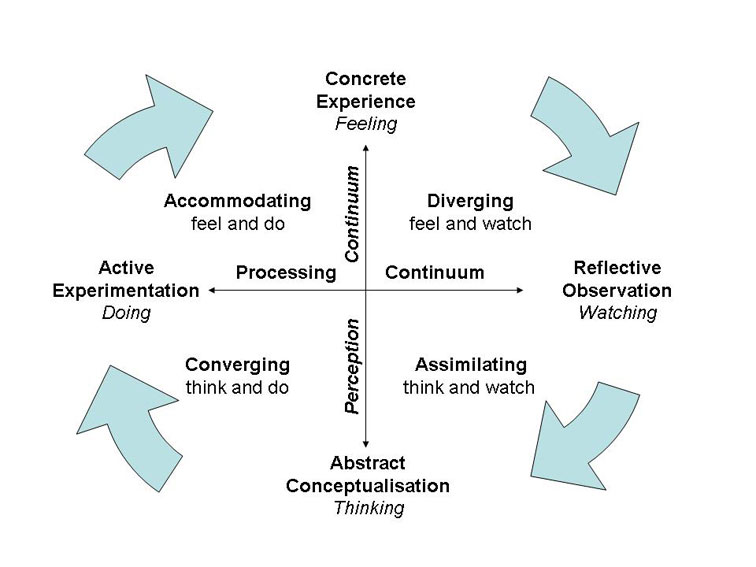
\includegraphics[width=0.4\textwidth]{kolb_diagram}
    \caption{Kolb's Experiential Learning Cycle}
    \label{fig:kolb_diagram}
\end{figure}

J. Goosby Smith's work, "Abstracting The Concrete, Concretizing The Abstract: Reframing Diversity Education Through Experiential Learning Theory," further explores this concept through the lens of Western diversity education. Smith critiques traditional approaches to diversity education for their reliance on the earlier stages of Kolb's learning cycle, which focuses on abstract conceptualization and reflective observation. Smith argues that these stages are insufficient for developing cultural competence, as they fail to provide students with the concrete experiences necessary for understanding and empathizing with diverse perspectives. Instead, Smith advocates for a more immersive and participatory approach to diversity education that exposes students to diverse perspectives and encourages them to engage with and reflect on these perspectives actively \cite{smith_abstracting_2011}. 

Integrating these ideas into a VR experience offers a few compelling advantages. Firstly, it allows educators to move beyond didactic teaching, providing students with dynamic environments to engage and reflect upon material actively through a pseudo-lived experience. Secondly, by emphasizing the importance of concrete experience, ELT encourages learners to critically examine their own beliefs as it becomes more difficult to ignore the lived experiences of others when you are all but physically placed into their shoes. Finally, applying ELT in this context helps address modern paradigms in education, such as critical thinking, empathy, and the ability to navigate complex social landscapes \cite{henderson_world_2000}.

By emphasizing the importance of concrete experience, VR can provide students with a more immersive and participatory learning experience, allowing them to engage with and reflect on religious material more dynamically and interactively. This approach can help students develop a deeper understanding of religious concepts and practices and a greater appreciation for the diversity of religious beliefs and traditions.

\section{VR as an Educational Tool}
The Meta Quest 3 is a standalone head-mounted display (HMD) that can produce high-quality VR experiences without needing a computer or external sensors. This makes it an ideal tool for educational settings, as it is portable and easy to set up. The Meta Quest 3 is also relatively affordable, making it accessible to various educational institutions \cite{quest_3}. The previous model, the Meta Quest 2, has already been tested for efficacy and, in some cases, outperformed its AR counterpart, the Microsoft HoloLens 2, in terms of user satisfaction and learning outcomes \cite{kyaw_comparing_2023}.

All this to say, VR has become an accessible tool to put users into a hyper-immersive environment, making it ideal for an educational setting where conveying ideas and the weight of said ideas is paramount.

For instance, An and Shin demonstrated how VR could significantly enhance early childhood traffic and life safety education by providing interactive and engaging learning experiences that convey these issues' importance more effectively than traditional methods \cite{an_teachers_2023}. Studies have also shown that these technologies not only increase engagement and motivation but also enhance knowledge retention, skill acquisition, and conceptual understanding—for example, Gleason et al. \cite{gleason_developing_2022} and Please et al. \cite{please_virtual_2024} demonstrated the effectiveness of VR in surgical training simulations significantly improved trainee's technical skills and confidence, underscoring the potential of VR to enhance learning outcomes in a variety of educational contexts.

Another significant takeaway from the breadth of these studies is that these solutions are globally viable, transcending language and class barriers. This review cites studies from the United States \cite{gleason_developing_2022}, South Korea \cite{an_teachers_2023}, the United Kingdom and Uganda, Australia, and Canada \cite{kyaw_comparing_2023}. This global applicability is particularly relevant for democratizing religious education, as it can help students develop a more nuanced understanding of religious beliefs and practices worldwide.

The study by Elena et al. \cite{elena_virtual_2022} offers a compelling insight into the persuasive power of virtual reality (VR) as a communication medium, especially in contexts where compliance and behavioral change are desired outcomes. Their research delved into the dynamics of VR-mediated interactions, comparing them to traditional face-to-face communication in scenarios requiring persuasion. The findings highlighted VR's unique capability to create immersive environments that can significantly influence users' perceptions and actions. This ability stems from VR's immersive nature, which can engender a heightened sense of presence and engagement, making the persuasive content more impactful than traditional settings. The implications of this study are profound, suggesting that VR can be an effective tool not only in educational contexts but also in areas such as health communication, environmental awareness, and social change initiatives. 

Despite its potential, integrating VR into educational settings is challenging. Across the board, the most significant issues impacting the efficacy of VR in educational settings are willingness and technical complexity \cite{peng_virtual_2020} \cite{gleason_developing_2022} \cite{gomindes_use_2023}.

\section{Case Study}
While we've seen the different ways an immersive experience has its benefits, challenges, and transformative potential, we can look at a few takeaways common to almost all of the studies that can best guide our approach to integrating VR into religious education.

\subsection{VR as a Tool for Comfort and Competence}
In studies where VR was used to teach new skills or further practice old ones, there often was no significant difference in learning outcomes between VR and traditional methods. However, the VR groups consistently reported lower stress and higher comfort from being inside the immersive experience \cite{gleason_developing_2022} \cite{please_virtual_2024}.

Gleason et al. found that VR simulations significantly improved trainees' technical skills and confidence, which was an extremely pertinent issue for the study as the trainees were medical students who had a limit on how much time they could spend in the operating room. By providing a realistic yet consequence-free environment, VR allows trainees to practice and repeat procedures, thereby reducing anxiety and building confidence before performing on actual patients. This psychological comfort translates into better preparedness and performance in basic surgical settings \cite{gleason_developing_2022} \cite{zaki_virtual_2023} \cite{buchori_virtual_2023}.

Similarly, in sports training, the study by Skopek et al. \cite{skopek_use_2023} highlighted VR's role in reducing performance anxiety among table tennis players. Through immersive practice sessions, players could focus on skill development without the immediate pressure of competition, leading to a more comfortable and confident approach during real matches.

Furthermore, García Fierros et al. \cite{garcia_fierros_virtualcpr_2021} research on VR-based CPR training illustrated how immersive simulations could decrease stress among participants learning life-saving techniques. The virtual environment provided a safe space for learners to practice and make mistakes, which is crucial in building competence and confidence in emergency medical responses.

The case of surgical learning in low- and middle-income countries (LMICs), as explored by Please et al. \cite{please_virtual_2024}, further underscores VR's capacity to enhance comfort and learning. By offering scalable and accessible training modules, VR has the potential to mitigate the stress associated with limited access to traditional surgical training resources in these regions.

The reduction of stress and enhancement of comfort through VR applications directly aligns with the broader objectives of our research, which seeks to explore innovative ways to deepen understanding and improve skill acquisition in religious diversity education. By leveraging VR's capacity to create comfortable, immersive learning environments, we can potentially transform the approach to teaching complex and sensitive subjects like religious diversity, making them more accessible and engaging for learners.

\subsection{VR as a Tool for Engagement}
Another common theme across the studies was VR's potential to increase engagement not through the unique affordances of the medium but simply the novelty it. When Please et al. \cite{please_virtual_2024} conducted their study training surgical residents in VR, they found that approximately 80\% of participants reported that the VR component of the conference considerably contributed to their reason to attend, even though they were learning and practicing lifesaving techniques \cite{please_virtual_2024}.

This novelty factor was also seen in the An and Shin study \cite{an_teachers_2023}, which was reported to be due to the age of the participants. The study was conducted with children aged 5-7, and the novelty of VR was a significant factor in their engagement. Similarly, Kyaw et al. \cite{kyaw_comparing_2023} found that the novelty of VR was a substantial factor in the attention of their participants, who were undergraduate students.

The implications of these findings are significant for our research, as they suggest that VR can be an effective tool for engaging students who otherwise may not have been interested in the subject or harbored enough interest to visit these significant sites on their own. By leveraging VR's novelty and immersive potential, we can potentially create engaging and accessible learning experiences that inspire students to explore and appreciate the rich tapestry of religious diversity.

\subsection{VR as a Tool for Creating Memorable Experiences}
The An and Shin study \cite{an_teachers_2023} found that VR was more effective than traditional methods in teaching early childhood safety education because the VR experience was more memorable. The study found that the VR group had a significantly higher recall of the safety rules they were taught than the traditional group. The students in the study were creating real memories of the experience, which made the learning more effective \cite{an_teachers_2023}.

Under illiberal right-wing rule, the Polish Ministry of Culture and National Heritage has invested in creating virtual reality films that depict significant events from Polish history in recent years. The study by Kazlauskaitė (2023) explores the profound impact of virtual reality (VR) on memory and perception within the context of Polish politics of memory. It delves into how VR, as a "technology of memory," shapes users' autobiographical memory, potentially manipulating their self-perception, beliefs, and social interactions according to the narrative created by VR developers. This research underscores the dual nature of VR as both an immersive educational tool and a potent medium for political and cultural influence, making it a critical point of reference for understanding VR's capacity to create memorable experiences that extend beyond traditional learning environments to influence collective memory and identity \cite{ruta_polish_2023}.

These findings, whether for better or for worse, show that VR tends to create memorable experiences that have the potential to shape our own autobiographical memory.

\section{The Intersection of VR and Experiential Learning}

Integrating the ELT framework with VR technology with advanced technology now seems to be a promising avenue for enriching students' learning experiences and reaching audiences who would not have previously resonated with the subject matter otherwise, specifically about religious education. The study by Li et al. \cite{li_religious_2023} is a pivotal example. Instead of VR, the team used an Augmented Reality (AR) application to enhance religious diversity education among elementary school students. Researchers conducted the study in a religiously diverse area of Taiwan during the Lantern Festival, a significant religious event. The AR application allowed students to explore the festival's spiritual significance and cultural practices, fostering a deeper understanding of religious diversity and cultural traditions. Their innovative approach showed improved attitudes toward different religions among students who used AR as part of their learning process compared to those who received traditional instruction.

This aligns closely with the principles of ELT, which emphasizes learning through experience. While not directly referenced, the ELT methodology was evidenced through the reflections conducted after the experiment, which showed that the students who used AR had a deeper understanding of the festival's spiritual significance and cultural practices through abstract conceptualization.

\section{Future Directions}

Building on the success of studies and reviews such as those by Li et al. \cite{li_religious_2023} and Please et al. \cite{please_virtual_2024}, we propose a framework for assessing future research in enhancing Buddhist education through VR simulations of the Swoyambhu Mahachaitya temple. The principles of ELT will guide this framework and aim to address the challenges and opportunities presented by using VR in religious education \cite{zhao_survey_2009}.

Here are some recommended metrics for future research based on the findings of this review:

\begin{enumerate}
    \item \textbf{Knowledge Assessment:} Pre- and post-intervention quizzes are critical for measuring learning gains related to religious diversity concepts through VR. Similar strategies were highlighted by Mayer \cite{Mayer_2020} in "Multimedia Learning," which underscores the effectiveness of tailored assessments in evaluating cognitive understanding in multimedia learning environments \cite{li_religious_2023} \cite{gleason_developing_2022}.
    \item \textbf{Attitudinal Surveys:} Student attitudes towards religions can be effectively gauged using Likert-scale surveys before and after VR interventions. Petty and Cacioppo's \cite{berkowitz_elaboration_1986} elaboration likelihood model, discussed in "Communication and Persuasion," supports using such surveys in measuring attitude changes resulting from persuasive communication, akin to immersive VR experiences. \cite{kyaw_comparing_2023}.
    \item \textbf{Engagement Metrics:} VR session logs provide valuable data on engagement, such as task duration and interaction rates. Dede's work \cite{Dede2009} supports the importance of these metrics research in "Immersive Interfaces for Engagement and Learning," which suggests that engagement metrics can significantly predict learning outcomes in immersive environments.
\end{enumerate}

\section{Conclusion}

This review has explored the transformative potential of VR in religious education, drawing on the principles of ELT and empirical studies to highlight the efficacy of VR in enhancing learning outcomes and engagement. The findings suggest that VR can be a powerful tool for creating immersive and participatory learning experiences that deepen students' understanding of religious diversity and cultural traditions. By leveraging VR's capacity to create comfortable, engaging, and memorable learning experiences, we can potentially transform the approach to teaching complex and sensitive subjects like religious diversity, making them more accessible and engaging for learners. The proposed framework for future research aims to build on these findings and address the challenges and opportunities presented by using VR in religious education, providing a roadmap for enhancing Buddhist education through VR simulations of the Swoyambhu Mahachaitya temple.

We are excited to see how this research will continue to evolve and contribute to the ongoing dialogue on enhancing educational practices and curriculum development in religious education.

\nocite{*}


\bibliography{litreview}
\bibliographystyle{IEEEtran}

\end{document}
